\documentclass{article}%
\usepackage[T1]{fontenc}%
\usepackage[utf8]{inputenc}%
\usepackage{lmodern}%
\usepackage{textcomp}%
\usepackage{lastpage}%
\usepackage[head=40pt,margin=0.5in,bottom=0.6in]{geometry}%
\usepackage{graphicx}%
%
\title{\textbf{Francia apoyó iniciativa para que CPI investigue crímenes en Venezuela}}%
\author{AFP}%
\date{29/09/2018}%
%
\begin{document}%
\normalsize%
\maketitle%
\textbf{URL: }%
http://www.el{-}nacional.com/noticias/mundo/francia{-}apoyo{-}iniciativa{-}para{-}que{-}cpi{-}investigue{-}crimenes{-}venezuela\_253731\newline%
%
\textbf{Periodico: }%
EN, %
ID: %
253731, %
Seccion: %
Mundo\newline%
%
\textbf{Palabras Claves: }%
Nicolás Maduro, Mundo, Gobierno\newline%
%
\textbf{Derecho: }%
18, %
Otros Derechos: %
5, %
Sub Derechos: %
5.1\newline%
%
\textbf{EP: }%
NO\newline%
\newline%
%
\textbf{\textit{Argentina, Canadá, Chile, Colombia, Paraguay y Perú enviaron una carta a la CPI para pedirle que investigue los crímenes contra la humanidad cometidos por el gobierno de Nicolás Maduro}}%
\newline%
\newline%
%
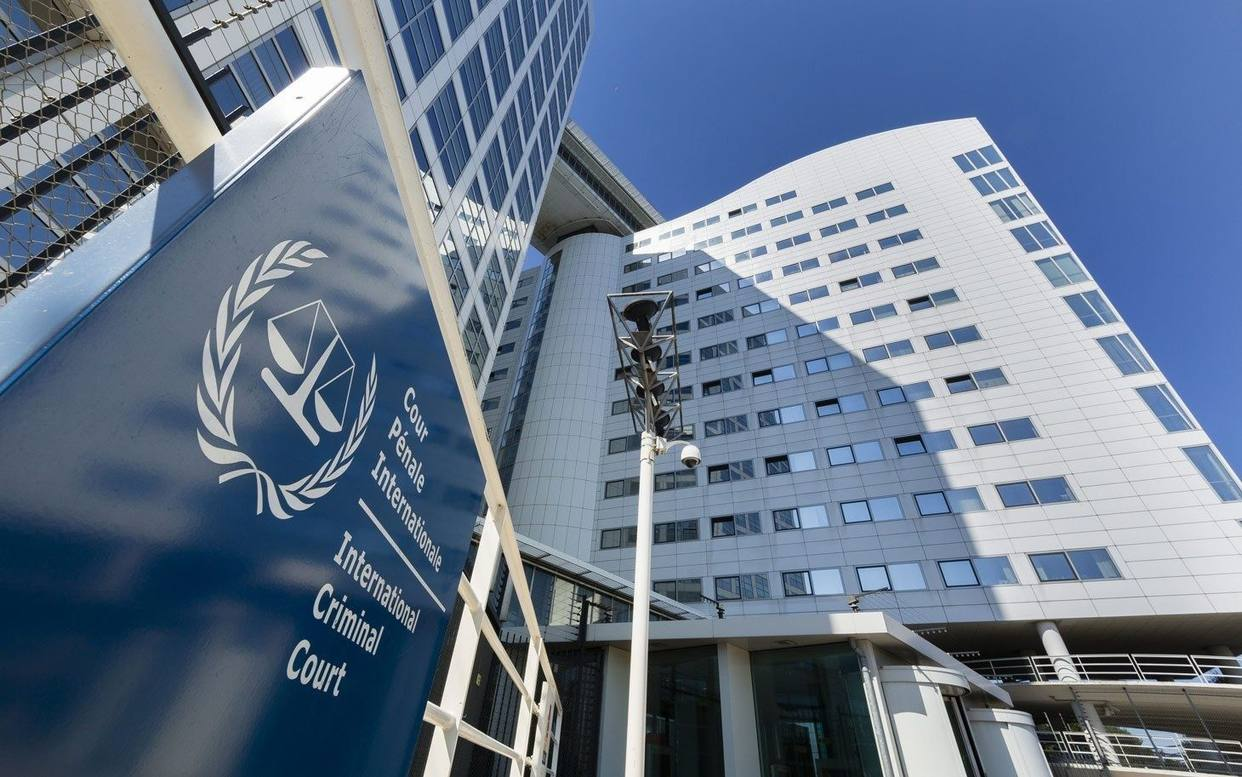
\includegraphics[width=300px]{212.jpg}%
\newline%
%
Francia expresó su apoyo a la iniciativa de cinco países de América Latina y Canadá que pidieron a la Corte Penal Internacional (CPI) que investigue al gobierno venezolano de Nicolás Maduro por crímenes de lesa humanidad, anunció el palacio de Elíseo.%
\newline%
%
"Francia considera que los esfuerzos de la Corte Penal Internacional tienen como naturaleza establecer los hechos que llevaron a esta crisis y, contribuir así a encontrar una salida", escribió la presidencia francesa en un comunicado.%
\newline%
%
Francia pide "encarecidamente a las autoridades venezolanas que inicien el diálogo con la oposición para restablecer el funcionamiento democrático de las instituciones, hallar una salida a la crisis política y contribuir a mejorar la economía venezolana", continúa el comunicado.%
\newline%
%
Argentina, Canadá, Chile, Colombia, Paraguay y Perú enviaron una carta a la CPI para pedirle que investigue los crímenes contra la humanidad cometidos según ellos por el gobierno de Nicolás Maduro.%
\newline%
%
En Venezuela hay denuncias serias de detenciones arbitrarias, asesinatos, ejecuciones extrajudiciales, torturas, abusos sexuales, violaciones, atentados flagrantes contra el debido proceso inclusive de algunos menores de edad, dijo el miércoles el canciller argentino, Jorge Faurie.%
\newline%
%
\end{document}